%%%%%%%%%%%%%%%%%%%%%%%%%%%%%%%%%%%%%%%%%%%%%%%%%%%%%%%%%%%%%%%%%%%%%%%%%%%%%%%%
%
% Setup
%

\documentclass[letterpaper,twocolumn,10pt]{article}
\usepackage{usenix}
\usepackage[bookmarks,colorlinks=true,citecolor=black,urlcolor=black,linkcolor=black]{hyperref}
\usepackage[rgb,dvipsnames]{xcolor}
\usepackage{xcolor}
\usepackage{xspace}
\usepackage{tcolorbox}
\usepackage{float}
\usepackage{subcaption}
\usepackage[hyphenbreaks]{breakurl}
\tcbuselibrary{listings}
\def\UrlBreaks{\do\/\do-}
\usepackage{printlen}
\uselengthunit{in}
\newlength\imageheight
\newlength\imagewidth

\newcommand{\eg}{{\em e.g., }}
\newcommand{\ie}{{\em i.e., }}
\newcommand{\paragraphb}[1]{\vspace{0.03in}\noindent{\bf #1} }
\newcommand{\paragraphe}[1]{\vspace{0.03in}\noindent{\em #1} }
\newcommand{\paragraphbe}[1]{\vspace{0.03in}\noindent{\bf \em #1} }

\newcommand{\eric}[1]{\textcolor{blue}{(ERIC: #1)}}
\newcommand{\ericf}[1]{\footnote{\textcolor{blue}{ERIC: #1}}}
\newcommand{\matt}[1]{\textcolor{red}{(MATT: #1)}}
\newcommand{\mattf}[1]{\footnote{\textcolor{red}{MATT: #1}}}
\newcommand{\oliver}[1]{\textcolor{green}{(OLIVER: #1)}}
\newcommand{\oliverf}[1]{\footnote{\textcolor{green}{(OLIVER: #1)}}}

\newcommand{\Yanc}{\textit{Yanc}\xspace}
\newcommand{\yanc}{\textit{yanc}\xspace}
\newcommand{\yancfs}{\textit{yancfs}\xspace}


\setlength{\pdfpagewidth}{8.5in}

\setlength{\pdfpageheight}{11in}


\begin{document}

%%%%%%%%%%%%%%%%%%%%%%%%%%%%%%%%%%%%%%%%%%%%%%%%%%%%%%%%%%%%%%%%%%%%%%%%%%%%%%%%
%
% Metadata
%


\title{Evaluation of the Tagged Up/Down Sorter Priority Queue} 

	\author{
		Michael Couglin
		\\
		University of Colorado, Boulder \\
%		\texttt{\{first.last\}@colorado.edu}
	}

	\maketitle


	\section{Introduction}
\label{sec:intro}

In this paper, I present an evaluation of the Tagged up/down sorter priority queue first presented by Moore, et. al. against other hardware priority queues for my final project for ECEN 5139 \cite{Moore95taggedup/down}. This evaluation is of the performance of this queue compared to the published results of other queues when implemented in an FPGA in terms of speed, queue size and resource utilization. This project was first motivated by the presentation of this particular priority queue during class and how it compares to other priority queues. Priority queues themselves are a classic example of a hardware task and as such, fall directly into the scope of computer-aided verification. Queuing is an important task that needs to be performed in many different applications, with a very frequent usage in networking, but is also used in other areas, including databases or even in some sorting applications \cite{huang2014scalable}.

The tagged up/down sorter queue that is the subject of this was first presented in 1995, but it appears to have not been used by the hardware community to any significant extent. However, the paper claims to achieve very good performance in both speed and resource utilization when implemented in hardware, so a comparison to the state-of-the-art solutions may reveal a potential new application of this queue, or a reason for why this solution is not used today. The primary works being used for comparison are the hybrid hardware-software priority queue presented by Kumar et. al. \cite{KumVya13B}, the hybrid BRAM-based tree priority queue presented by Huang et. al., and a canonical priority queue implemented as a min-heap as a baseline. The first two of these implementations are from very recent publications, both published in 2014, and so can be considered examples of the state-of-the-art of this field.

An analysis of the tagged up/down sorter compared to the two state-of-the-art solutions shows a theoretical advantage in performance, as this queue is able to achieve enqueue/dequeue operations in a single FPGA cycle, whereas the state-of-the-art solutions only claim "nearly" one cycle performace (in the case of Huang et. al.) \cite{huang2014scalable}. In addition, both of these solutions  claim low resource utilization compared to other solutions when implemented in an FPGA, whereas the tagged up/down sorter was only tested in simulation. Therefore, an analysis of both the performance and utilization may yield insight into the potential trade-offs for using each solution.

In the remainder of this paper, I will present my evaluation methodology (Section \ref{sec:method}), the results of the evaluation (Section \ref{sec:eval}), a discussion of these results (Section \ref{sec:discussion}), and finally, a conclusion (Section \ref{sec:conclusion}).
	\section{Evaluation Methodology}
\label{sec:method}

In order to evaluate this queue against the performance of state-of-the-art designs, I required an implementation of the queue that can be programmed to an FPGA, a testbench to evaluate the performance of the queue and an FPGA device to target and use for the evaluation. For the implementation of the queue, I used Vivado High-level synthesis (HLS) to implement the queue using C++ and then have it synthesized to hardware, as well as a Verilog implementation provided by Professor Somenzi for a direct hardware implementation. I also used an HLS and Verilog implementation of a min-heap priority queue for the baseline. I chose to use HLS partly due to my familiarity with this particular tool and my lack of experience with Verilog, and partly because these algorithms are generally only expressed in software programming languages (there are, in fact, no easy-to-find implementations of hardware min-heap and few accessible priority queue implementations in general).

For the FPGA used for evaluation, I chose the Zedboard evaluation board, as this board was accessible to me from prior research. This board includes a Zynq7000 SoC, which incorporates an ARMv7 dual-core CPU and a 7000-series FPGA, allowing for a Linux OS to be able to access and program the FPGA. Using this capability, I instantiated a testbench hardware module in the FPGA along with a particular queue implementation that runs the same test on each queue, referred to as the "runner." This module then returns the results of this test to a program running in the operating system as the number of enqueue operations performed. The software application in the OS accesses this module as a memory-mapped peripheral and records the time to execute the test, as well as the result returned by the module. The runner itself runs a test to enqueue as many elements as possible with incrementing and random priorities, and dequeue these items until the queue is empty, repeatedly for 10,000 iterations. The number of iterations is important, as there is significant overhead when interfacing with the runner module from software, so the FPGA needs to execute a time-consuming operation in order for it to be measurable. Due to time constraints, only a single queue size was used for each evaluation, as the queue size must be specified before synthesis and is time consuming to repeat.

Evaluation of the resource utilization of this queue is much more straight-forward, as utilization metrics are an output of synthesis. Therefore, each design only needs to be synthesized with different queue sizes to determine the utilization metrics. These output metrics are then compared to the published results of the state-of-the-art implementations.
	\section{Evaluation}
\label{sec:eval}

\subsection{Resource Utilization}
For evaluation of the resource utilization of the different implementations, the min-heap and tagged up/down sorted were synthesized with various different queue sizes until the required resources exceeded the resources available in the FPGA. The results were then compared with the published results of the state-of-the-art implementations. After performing these steps, it was clear that the resources in contention were the look-up tables (LUTs), flip-flops (sometimes known as slice registers) and block RAMs(BRAMs). Since these implementations generally do not need to interface with external devices, usage of only these resources is expected, as the modules are only operating in the FPGA. In addition, since these are not digital signal processing applications, but are highly combinatorial and memory-intensive, high usage of LUTs and BRAMs is also expected. However, it should be noted that the min-heap and tagged up/down sorter priority queues do not use any BRAM resources, as they only store the priorities with no associated data. Since the other queue implementations do store extra data, they make us of the BRAMs, so BRAM utilization is not analysed.

\begin{figure}[t!]
	\centering
	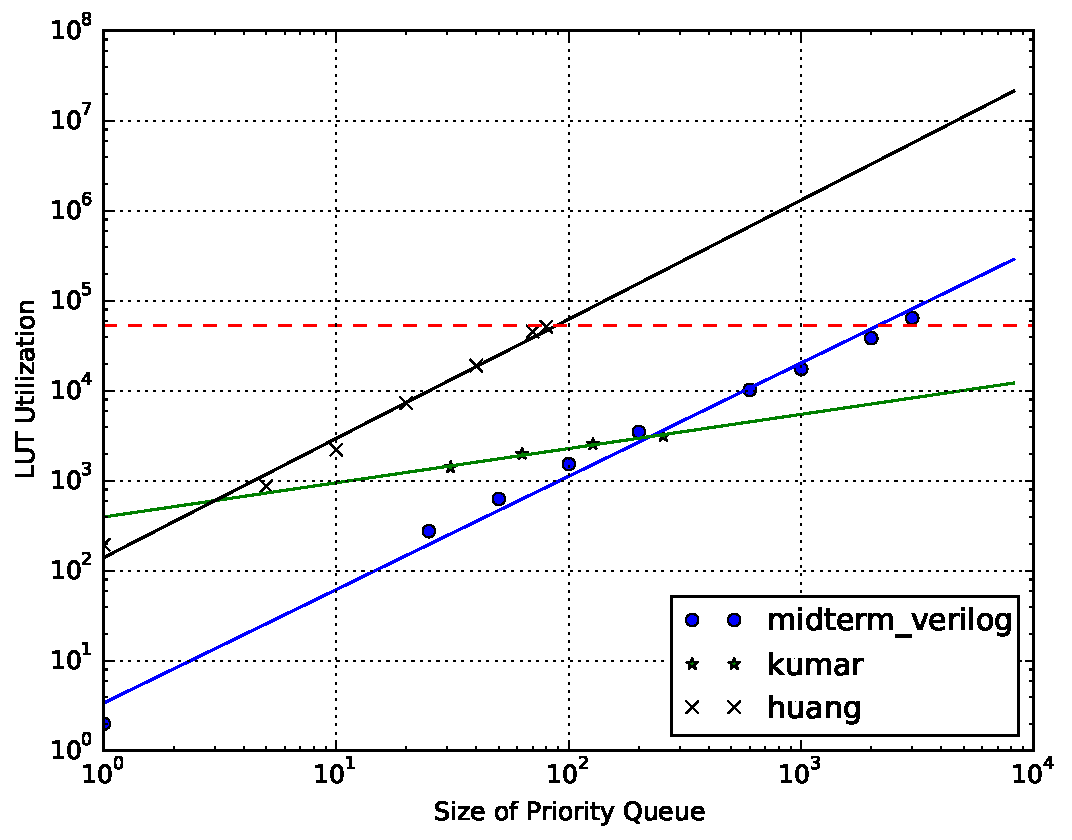
\includegraphics[width=\columnwidth]{data/lut_utilization.pdf}
	\caption{LUT Utilization}
	\label{fig:luts}
\end{figure}

\begin{figure}[t!]
	\centering
	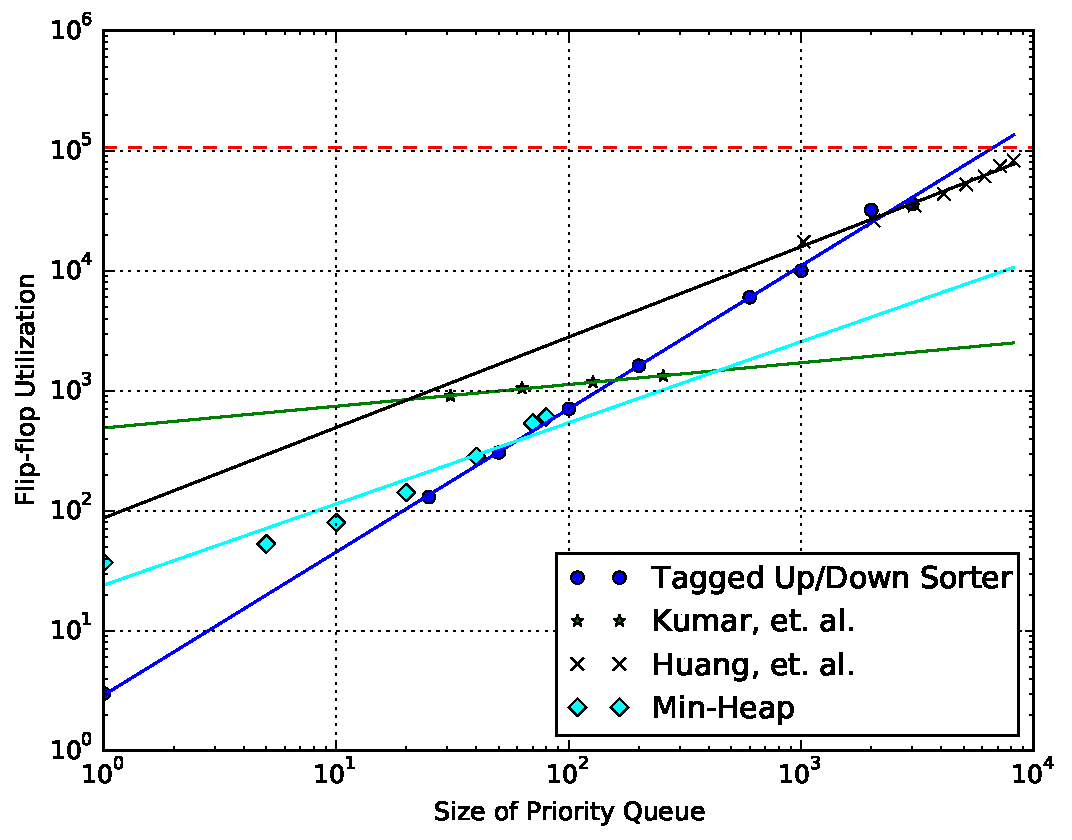
\includegraphics[width=\columnwidth]{data/ff_utilization.pdf}
	\caption{Flip-flop Utilization}
	\label{fig:ffs}
\end{figure}

The resource utilization of LUTs and flip-flops are depicted in Figure \ref{fig:luts} and Figure \ref{fig:ffs} respectively, with the dashed line marking the resource limit of the Zedboard. It can be seen that all of the different implementations are approximately linear in their resource utilization, but a shallower slope indicates slower resource usage as queue size increases. It should also be noted that the published results for the state-of-the-art implementations only provided a small set of data points, so a linear regression is fit to the published data for comparison. Also, the hybrid queue proposed by Huang et. al. only provides resource utilization of flip-flops and BRAMs, and then, only as percentages of their test device's total resources (the ZC706 evaluation board). After extrapolating the flip-flop usage from their published data, this metric can be used for comparison, but LUT usage for this implementation cannot be compared.

\begin{figure}[t!]
	\centering
	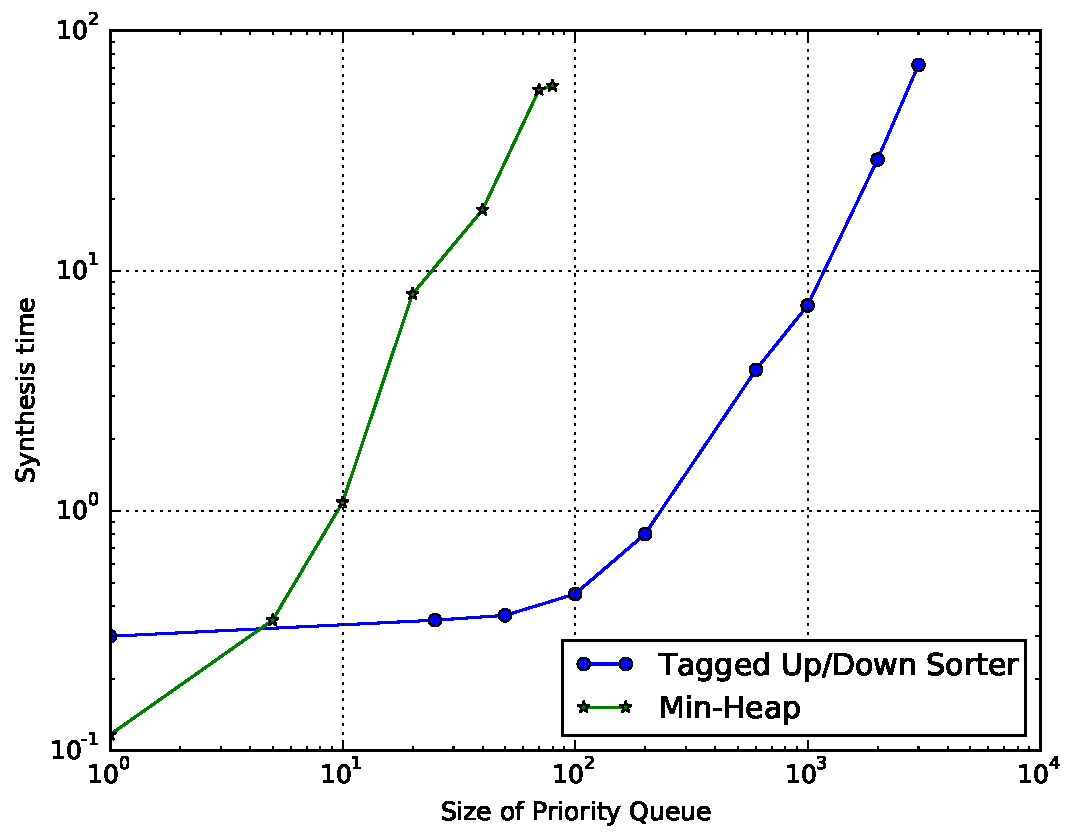
\includegraphics[width=\columnwidth]{data/synthesis_times.pdf}
	\caption{Synthesis Times}
	\label{fig:synth_times}
\end{figure}

In addition to these utilization numbers, I also present a plot of the time required for synthesis of each of the queue sizes to complete for the min-heap and the tagged up/down sorter for each queue size in Figure \ref{fig:synth_times}. From this plot, it can be seen that the time for synthesis increases quickly with the queue size, and is part of the reason for the limited performance results that I am able to present.

\subsection{Performance}
Performance is difficult to compare, since both of the published state-of-the-art implementations report performance in different ways. In addition, there is a lower bound of performance in that an operation cannot be performed faster than an FPGA clock cycle, since the queue is implemented with clock flip-flops. However, as the Tagged Up/Down sorter is implemented in Verilog to perform an enqueue or dequeue operation in a single clock cycle, it theoretically outperforms the state-of-the art solutions, as neither achieve this performance in both cases.

The in-hardware testbed, as previously described, performs 10,000 iterations of a series of enqueue and dequeue operations. The queue that is uses is of size 40, since this is the largest queue that able to successfully access when the queue was implemented as a min-heap. The performance results of the two different implementations is tabulated in Table \ref{tab:perf}. It should be noted that repeated execution of the testbed and software interface yield the same results, since the testbed is a deterministic hardware function. Also, the testbed detects that the min-heap is not implemented correctly, as the output of the queue does not seem to be correct, even though the queue passed simulation. However, the time to perform a single enqueue or dequeue operation should not be affected.

As can be seen from the performance results, the min-heap and Tagged Up/Down sorter achieve the same performance. This is because they both can perform an operation in a single cycle, and so cannot run any faster. Therefore, their performance is solely determined by the clock frequency of the FPGA.

\begin{table}[t!]
	\centering
	\small
	\resizebox{\columnwidth}{!}{
	\begin{tabular}{| c | c | c |}
		\hline
		Queue Implementation & Test Execution Time & Number of Operations \\ \hline
		Tagged Up/Down Sorter & 28002 $\mu$s & 140,000 \\ \hline
		Min-Heap & 27799 $\mu$s & 140,000  \\ \hline
	\end{tabular}
	}
	\caption{Performance Results}
	\label{tab:perf}
\end{table}





	\section{Discussion}
\label{sec:discussion}

After

	

%%%%%%%%%%%%%%%%%%%%%%%%%%%%%%%%%%%%%%%%%%%%%%%%%%%%%%%%%%%%%%%%%%%%%%%%%%%%%%%%
%
% References
%

	\footnotesize
	\bibliographystyle{abbrv}
	\bibliography{refs,refs2}

\end{document}

% vim: set noet : %
